\section{Robustly disjoint sr-paths}
\label{section:rdp}

In this section we propose a technique to leverage segment routing to provide a failure
tolerant disjoint path service. The idea is to connect two sites via a pair of 
disjoint sr-paths like we did in the previous section and ensure these sites remain connected by two disjoint paths
even in case of a link failures. Segment routing is interesting in such
a setting because, since it is based on shortest path routing, after a set
of network links goes down, these sr-paths will automatically converge towards new paths on $G$
as the routers update theirs routing tables. 

The idea is thus to take this into account when building the sr-paths and 
make sure that the set of paths on $G$ that correspond the sr-paths are disjoint
after IGP re-convergence for any given failure. If we manage to compute such paths, then we have the guarantee
that our solution remains disjoint even in case something goes wrong.

Concretely, we will assume that a set of failure that we want to support is
given as input and we will seek pairs of paths that are tolerant to any 
failure in the given set.

\begin{definition}
Let $G$ be a network. A \emph{failure set} is a set $F = \{f_1, \ldots, f_m\}$ such that
for all $i$, $f_i \subseteq E(G)$ and $\emptyset \in F$.
\end{definition}

Requiring that the empty set belongs to the failure sets poses no practical restriction
and is there just to make the following definitions more elegant.

If we want to support single link failures we can set $F = \{ \{ e \} \mid e \in E(G) \} \cup \{ \emptyset \} = F_E(G)$.
If we know specific shared risk link groups~\cite{ghobadi-imc16,turner2010california} we can also add
them to $F$ so that our paths become failure tolerant to them.
Note that there are limits to the amount of failures that one can add to $F$. If we add too many
failure sets then we have a high chance of over constraining the problem and making it have no
admissible solution.

We model a failure of a set of edges $f \in F$ as removing those edges from the network. Therefore
it can happen that the network becomes disconnected after a failure occurs. This can lead to the fact
that the sr-paths might become undefined if they either require to route traffic between disconnected parts of the network
or they use an adjacency segment over an element of $f$. In particular, this means that we cannot use adjacency segments
over any link belonging to an edge in $F$ since such a failure would make the path unusable. As a consequence,
if $F = F_E(G)$ then we cannot use adjacency segments at all. This leads to the following definition.

%For this reason,
%we will simply ignore adjacency segments in this section and consider only paths with node segments only.

\begin{definition}
Let $G$ be a network, $\sr{p} = \langle x_1, \ldots, x_n \rangle$ a sr-path on $G$ and $F$ a failure set. We say that $\sr{p}$ is \emph{well defined
with respect to $F$} if $\sr{p}$ does not contain any adjacency segment belonging to a set $f \in F$
and for each $i = 2, \ldots, n$ and $f \in F$, $G \setminus f$ contains at least one path from $x^2_{i - 1}$ to $x^1_i$.
\end{definition}

Figure \ref{fig:welldefined} illustrates this definition. Suppose that the failure set $F$ contains a failure set $f$ whose
elements consist of all edges touching node $\node{i}$ (in both directions). Then any path using node $\node{i}$ as a segment
will not be well defined with respect to $F$. For instance, $\sr{p} = \langle \node{a}, \node{g}, \node{i}, \node{h} \rangle$
will fail to forward packets from $\node{g}$ to $\node{i}$ if failure $f$ occurs.
This example also illustrates another important aspect of robustly disjoint paths. Imagine that we want to consider node failures
and also have disjoint sr-paths that are tolerant to node failures. We can model a node failure with a failure set $f$ consisting
of all edges incident to that node (in both directions). However, this will imply that that node becomes a forbidden node segment for
any sr-path in the solution. A corollary of this is that it is impossible to have robustly disjoint paths that are tolerant to the failure of
\emph{any} node since this would prevent any sr-path to contain segments altogether.

\begin{figure}
\begin{center}
\begin{tikzpicture}
\def\x{0}
\def\y{0}

\node[scale=0.15] (a) at (0.5 + \x,  0.5 + \y) {\router{a}{marked}};
\node[scale=0.15] (b) at (0.5 + \x, -1.0 + \y) {\router{b}{router}};
\node[scale=0.15] (c) at (2.5 + \x,  0.0 + \y) {\router{c}{router}};
\node[scale=0.15] (d) at (4.5 + \x,  0.0 + \y) {\router{d}{router}};
\node[scale=0.15] (e) at (4.0 + \x, -2.0 + \y) {\router{e}{router}};
\node[scale=0.15] (g) at (6.0 + \x,  0.5 + \y) {\router{g}{marked}};
\node[scale=0.15] (i) at (8.0 + \x,  0.0 + \y) {\router{i}{marked}};
\node[scale=0.15] (h) at (7.0 + \x, -1.5 + \y) {\router{h}{marked}};
\node[scale=0.15] (f) at (4.0 + \x, -3.5 + \y) {\router{f}{router}};
\node[scale=0.15] (j) at (8.0 + \x, -2.5 + \y) {\router{j}{router}};
\draw[line width=2] (a) edge[above, sloped] node[black] {} (b);
\draw[line width=2]  (a) edge[above, sloped] node[black] {} (c);

\draw[line width=2] (b) edge[above, sloped] node[black] {} (c);
\draw[line width=2] (b) edge[above, sloped] node[black] {} (e);
\draw[line width=2] (b) edge[above, sloped] node[black] {} (f);
\draw[line width=2]  (c) edge[above, sloped] node[black] {} (d);
\draw[line width=2]  (d) edge[above, sloped] node[black] {} (e);
\draw[line width=2]  (d) edge[above, sloped] node[black] {} (g);
\draw[line width=2] (e) edge[above, sloped] node[black] {} (c);
\draw[line width=2] (e) edge[above, sloped] node[black] {} (f);
\draw[line width=2] (f) edge[above, sloped] node[black] {} (j);
\draw[line width=2] (f) edge[above, sloped] node[black] {} (h);
\draw[line width=2, red] (g) edge[above, sloped] node[black] {} (i);
\draw[line width=2]  (g) edge[above, sloped] node[black] {} (h);
\draw[line width=2] (h) edge[above, sloped] node[black] {} (j);
\draw[line width=2, red] (i) edge[above, sloped] node[black] {} (h);
\draw[line width=2]  (e) edge[above, sloped] node[black] {} (h);

\draw[line width=3, darkgreen]  (a) edge[above, bend left=15, sloped, ->] node[black] {} (c);
\draw[line width=3, darkgreen]  (c) edge[above, bend left=15, sloped, ->] node[black] {} (d);
\draw[line width=3, darkgreen]  (d) edge[above, bend left=15, sloped, ->] node[black] {} (g);
\draw[line width=3, darkgreen]  (g) edge[above, bend left=15, sloped, ->] node[black] {} (i);
\draw[line width=3, darkgreen]  (i) edge[above, bend left=15, sloped, ->] node[black] {} (h);

\node[draw, fill=green!50!white, above = 0.1cm of a] (y1) {\small $x_1$};
\node[draw, fill=green!50!white, above = 0.1cm of g] (y2) {\small $x_2$};
\node[draw, fill=green!50!white, above = 0.1cm of i] (y3) {\small $x_3$};
\node[draw, fill=green!50!white, right = 0.1cm of h] (y3) {\small $x_4$};

\end{tikzpicture}
\end{center}
\caption{The sr-path $\langle \node{a}, \node{g}, \node{i}, \node{h} \rangle$ is not well defined if edges 
$\edge{g}{i}$, $\edge{i}{g}$, $\edge{i}{h}$, $\edge{h}{i}$ are in $F$.}
\label{fig:welldefined}
\end{figure}


We can now define the robustly disjoint paths (RDPs).

\begin{definition}
Let $G$ be a network, $\sr{p}_1$, $\sr{p}_2$ be two sr-paths and $F$ a failure set. We say that
$\sr{p}_1$ and $\sr{p}_2$ are \emph{robustly disjoint} if they are disjoint and well defined
on $G \setminus f$ for every $f \in F$.
\end{definition}

You can see that this definition also ensures that robuslty disjoint paths are 
disjoint to begin with since we assume that $\emptyset \in F$.

\begin{problem}{Robustly disjoint sr-path problem}
\label{prob:rdp}
\textbf{Input:} A network $G$, a failure set $F$, $s_1, s_2, t_1, t_2 \in V(G)$ and $k \in \mathbb{N}$.

\textbf{Output:} Two robustly disjoint sr-paths $\sr{p}_1 \in \Pk(s_1, t_1)$, $\sr{p}_2 \in \Pk(s_2, t_2)$ with respect to $F$.
\end{problem}

Since Problem \ref{prob:disjointsrp} is \NPhard, this problem must also be since we get the same problem
by setting $F = \{ \emptyset \}$.

It is not hard to adapt the disjoint sr-path MIP model proposed in the previous section 
to the case of robustly disjoint paths as well as our dedicated algorithm as we will show in the
remainder of this section.

\subsection{Adapting $\sredp$ to RDPs}

Adapting model $\sredp(G, s_1, s_2, t_1, t_2)$ to support robustly disjoint paths
is very simple. The only thing that we need to change are the disjointness constraints
so that they take the failures into account.

Recall that we ensure disjointness by requiting that if $e \in E(\sp(u, v))$ then
at most one of $x^1_{uv}, x^2_{uv}$ is set to $1$. To ensure that the sr-paths 
are robuslty disjoint we need to ensure that if
$$
e \in \bigcup_{f \in F} E(\sp(G \setminus f, u, v))
$$
then at most one of $x^1_{uv}, x^2_{uv}$ is equal to $1$.

For this we define a new indicating function $I_F$ such that $I_F(u, v, e) = 1$
if and only if $e$ belongs to the shortest paths between $u$ and $v$ 
on $G \setminus f$ for some $f \in F$. The robuslty disjoint path model
are obtained by replacing $I$ by $I_F$.

The cost of this adaptation is of course that pre-computing these $I_F$ functions takes more time,
specially if $F$ is very large. However, this is only needed to be done once. We can build the model
once and only adapt it for the specific sources and destinations before each computation. Using the MIP model
is also more flexible and can easily be extended to compute more than two paths. 

\subsection{Adapting the dedicated algorithm to RDPs}

Algorithms \ref{algo:disjoint_srp} and \ref{algo:disjoint_srp_dfs} are also easily adaptable
to the case of robuslty disjoint paths but this results in a very inefficient algorithm.
The problem is that checking whether the paths are disjoint after any failure requires 
$|F|$ bit set comparisons meaning that each step of the algorithm is $|F|$ times slower.
For completeness we will describe the needed modifications on the algorithms.

To ensure that the sr-paths computed by the algorithm are well defined, 
we need to prevent the algorithm from using consecutive node segments $u, v$ such that 
there is no path from $u$ to $v$ in $G \setminus f$. Also, we need to forbid any adjacency 
segment over an edge belonging to some $f \in F$. Both these steps can be achieved by
pre-computing the pairs of nodes that cannot appear as consecutive segments and 
preventing to use adjacency segments on the set $\{ e \in f \mid f \in F\}$. Contrary to the
next modification, this only slows down the preprocessing step of the algorithm, not the
algorithm itself.

What really slows down the algorithm is that we need to also ensure disjointness after any failure $f \in F$ occurs.
To avoid having to make $|F|$ shortest path computations we can pre-compute
$\sp(G \setminus f, u, v)$ for all $f \in F$ and $u, v \in V(G)$. Now instead of checking
for intersection between $E(\sr{p}_1)$ and $E(\sr{p}_2)$ we need to check 
for intersection for every $f \in F$. This is the reason why the algorithm is 
not usable in practice for generic failures unless $F$ is quite small. Note that this is not the case for the
MIP adaptation above, we need more time to build the model because of the
indicating function $I_F$ takes longer to compute but that is not really a problem
since it needs to be done only once for any given topology. We will see however
in the next sections that if $F = F_E$ (single-link failures) then we can
still obtain a fast algorithm.

\subsection{The case of single-link failures}

Recall from the above discussion that the bottleneck in adapting 
Algorithms \ref{algo:disjoint_srp} and \ref{algo:disjoint_srp_dfs} to the case of 
robustly disjoint paths is checking whether the paths are disjoint for every failure.
We are going to see how we can check this efficiently when the set of failures is the 
set of edges thus showing that computing robustly disjoint paths that are tolerant to 
single-link failures can be done efficiently in practice.

The idea is that we will aggregate all the edges in $\sp(G \setminus f, u, v)$ for all $f \in F$
into a single set that we call \emph{failure set}. And then we show that checking for intersection
between the failures sets is enough to ensure robustness when $F = F_E$.

\begin{definition}
Let $G$ be a network and $\sr{p} = \langle x_1, \ldots, x_n \rangle$ a sr-path on $G$. We define the \emph{failure set of $\sr{p}$}
as
$$
\fail(\sr{p}) = \bigcup_{f \in F_G} E(G \setminus f, \sr{p})
$$
%$$
%\fail(\sr{p}) = \left( \bigcup_{e \in E(G)} \bigcup_{i = 2}^n E(\sp(G \setminus e, x^2_{i - 1}, x^1_i)) \right) \cup \bigcup_{i : x_i \in E(G)} x_i
%$$
\end{definition}

The next result is a very simple lemma that states that a failure on an edge that is not used by a sr-path does not affect it. This is quite an
obvious result but it is important for the theorem that follows.

\begin{lemma}
\label{lemma:outside-edge}
Let $G$ be a network and $\sr{p}$ a sr-path on $G$. If $e \in E(G) \setminus E(\sr{p})$ then $E(G \setminus e, \sr{p}) = E(G, \sr{p})$.
\end{lemma}

\begin{proof}
Let $e \in E(G) \setminus E(\sr{p})$ and write $\sr{p} = \langle x_1, \ldots, x_n \rangle$. Since $e \notin E(\sr{p})$ we have 
that for each $i \in \{2, \ldots, n\}$, $\sp(G, x^2_{i - 1}, x^1_{i}) = \sp(G \setminus e, x^2_{i - 1}, x^1_{i})$. Also, $e$ cannot be an
adjacency segment of $\sr{p}$ or else it would belong to $E(\sr{p})$. Therefore,
\begin{align*}
E(G \setminus e, \sr{p}) & = \left( \bigcup_{i = 2}^n E(\sp(G \setminus e, x^2_{i - 1}, x^1_i)) \right) \cup \bigcup_{i : x_i \in E(G) \setminus e} x_i \\
& = \left( \bigcup_{i = 2}^n E(\sp(G, x^2_{i - 1}, x^1_i)) \right) \cup \bigcup_{i : x_i \in E(G) } x_i \\
& = E(G, \sr{p}).
\end{align*}
\end{proof}

The following theorem shows how we can efficiently check disjointness conditions for every failure in the case of single-link
failures.

\begin{theorem}
\label{thm:single-link}
Let $G$ be a network and $\sr{p}_1, \sr{p}_2$ be two sr-paths on $G$. Then $\sr{p}_1, \sr{p}_2$ are robustly
disjoint with respect to $F_E$ if and only if they are well defined, $\fail(\sr{p}_1) \cap E(\sr{p}_2) = \emptyset$ and 
$E(\sr{p}_1) \cap \fail(\sr{p}_2) = \emptyset$.
\end{theorem}

\begin{proof}
$(\Rightarrow)$ Suppose that $\sr{p}_1, \sr{p}_2$ are robustly disjoint. 
Thus for each $f \in F_E$ we have $E(G \setminus f, \sr{p}_1) \cap E(G \setminus f, \sr{p}_2) = \emptyset$.
Since $\emptyset \in F_E$ we have in particular that $\sr{p}_1$ and $\sr{p}_2$ are disjoint on $G$. Suppose that $\fail(\sr{p}_1) \cap E(\sr{p}_2) \neq \emptyset$.
Then there exists $e \in E(G, \sr{p}_1)$ such that $E(G \setminus e, \sr{p}_1) \cap E(G, \sr{p}_2) \neq \emptyset$. Since the paths are disjoint, 
it cannot be the case that $e \in E(G, \sr{p}_2)$. Therefore, by Lemma \ref{lemma:outside-edge} we have that $E(G \setminus e, \sr{p}_2) = E(G, \sr{p}_2)$.
This means that $E(G \setminus e, \sr{p}_1) \cap E(G \setminus e, \sr{p}_2) = E(G \setminus e, \sr{p}_1) \cap E(G, \sr{p}_2) \neq \emptyset$ contradicting the
fact that the sr-paths are robustly disjoint. The case where $E(\sr{p}_1) \cap \fail(\sr{p}_2) \neq \emptyset$ is analogous.

$(\Leftarrow)$ Suppose that $\sr{p}_1, \sr{p}_2$ are well defined and that $\fail(\sr{p}_1) \cap E(\sr{p}_2) = \emptyset$ and 
$E(\sr{p}_1) \cap \fail(\sr{p}_2) = \emptyset$. Assume that the paths are not robustly disjoint for $F_E$. Since they are well defined, 
this means that either $E(\sr{p}_1) \cap E(\sr{p}_2) \neq \emptyset$ or
there exists $e \in E(G)$ such that $E(G \setminus e, \sr{p}_1) \cap E(G \setminus e, \sr{p}_2)$. Since $\emptyset \in F_G$ we have
that $E(\sr{p}_1) \subseteq \fail(\sr{p}_1)$ and thus $E(\sr{p}_1) \cap E(\sr{p}_2) \subseteq \fail(\sr{p}_1) \cap E(\sr{p}_2) = \emptyset$. Then, let $e$ be such that
$E(G \setminus e, \sr{p}_1) \cap E(G \setminus e, \sr{p}_2) \neq \emptyset$. Since $E(\sr{p}_1) \cap E(\sr{p}_2) = \emptyset$, $e$ cannot belong to both
$E(\sr{p}_1)$ and $E(\sr{p}_2)$. If it does not belong to $E(\sr{p}_1)$ then by Lemma \ref{lemma:outside-edge} we have 
$E(G \setminus E, \sr{p}_1) = E(\sr{p}_1)$ so 
$\emptyset \neq E(G \setminus e, \sr{p}_1) \cap E(G \setminus e, \sr{p}_2) = E(\sr{p}_1) \cap E(G \setminus e, \sr{p}_2) \subseteq E(\sr{p}_1) \cap \fail(\sr{p}_2) = \emptyset$
which is a contradiction. The other case is analogous and also leads to a contradiction. It follows that the paths are robustly disjoint.
\end{proof}

Using Theorem \ref{thm:single-link} we can transfer the time it takes for checking whether paths remain disjoint to
a pre-computation step where we compute the failure sets defined above for each two nodes $u, v \in V(G)$. Using these 
we can incrementally build the failure sets as we build $\sr{p}_1$ by noting that if $\sr{p}_1 = \langle x_1, \ldots, x_n \rangle$ then
$$
\fail(\sr{p}) = \left( \bigcup_{i = 2}^n \fail(\langle x^2_{i - 1}, x^1_i \rangle) \right) \cup \bigcup_{i : x_i \in E(G)} x_i.
$$

Therefore, whenever we extend $\sr{p}_1 = \langle x_1, \ldots, x_n \rangle$ with a segment $x$, we simply need to make 
the union of the current failure set with the precomputed failure set $\fail \langle x^2_n, x \rangle$ and $x_i$ if $x_i$
is an adjacency segment. Again, because of the use of bitset, this is a lightweight operation.

These only need to be pre-computed once for each given topology. We propose an efficient algorithm that is able to
compute them in under a minute even on the largest topologies. Thus it is 
reasonable to recompute them whenever the topology changes as these do not happen every minute.

% We already briefly mentioned above where the changes need to be applied in the algorithm for implementing robustness. For completeness we 
% will explicitly show the changes for the case of single-link failures.
% 
% \todo{complete this}

\subsubsection{Pre-computing the failure sets}

As we showed above, the failure sets for single-link failures are composed of the failure sets of the sr-path $\langle x, y \rangle$.
We are now going to describe how we can compute these efficiently. If we followed the definition we would loop over all pairs $x, y \in V(G)$ and
edges $e \in E(G)$ and for each edge we would compute the shortest path subnetwork from $x$ to $y$ on $G \setminus e$. 
However this is very costly. Instead, we can take advantage of Lemma \ref{lemma:forwdp}. For each fixed $x$ and $e \in E(G)$ we will compute the
shortest path subnetwork rooted at $x$. Then we compute a topological order of it and use Equation (\ref{eq:forwdp}) to compute
$E(\sp(G \setminus e, x, y))$.

We also add two ideas to accelerate the algorithm. The first is based on Lemma \ref{lemma:outside-edge}. It simply consists of ignoring
sets $e \notin E(\sp(x, y))$ since these will not add any new edges to $\fail \langle x, y \rangle$. The second idea is that we can ignore edges that
belong to an ECMP component between $x$ and $y$ since removing them will also not contribute to any new shortest paths because there will
always be at least one of the previous shortest paths that remains after the removal of $e$.
A formalization of this is provided as Algorithm \ref{algo:prefail}.

\begin{algorithm}[t]
\small
\caption{$\textsf{precompute-failEdges}\left( G, \sp, fwe \right)$}
\begin{algorithmic}[1]
\FOR{$u, v \in V(G)$}
  \STATE $\fail(u, v) \gets fwe(u, v)$
\ENDFOR
\FOR{$u \in V(G)$}
  \cmtline{optim 1: only consider edges in $\sp(u)$ as the others have no effect}
  \FOR{$f \in E(\sp(u))$}
    \cmtline{optim 2: check degree to consider only edges not in ECMP components}
    \IF{$\delta^-(\sp(u), f^2) \leq 1$}
      \STATE $\sp(f, u) \gets \textsf{dikstra-dag}(G \setminus f, u)$
      \STATE $order \gets \textsf{toposort}(\sp(u))$
      \FOR{$v \in order$}
	\FOR{$e \in \ine(\sp(u), v)$}
	  \STATE $\fail(u, v) \gets \fail(u, e^1) \cup \{ e \}$
	\ENDFOR
      \ENDFOR
    \ENDIF
  \ENDFOR
\ENDFOR
\RETURN $\fail$
\end{algorithmic}
\label{algo:prefail}
\end{algorithm}

\subsection{Evaluation of RDPs}

\subsubsection{Evaluating effective robustness of RDP}

Using the above concepts we can compute pairs of sr-paths that are robustly disjoint to single-link failures.
This is what our theoretical results guarantee. However, it could very well be the case that our paths are actually
robust to a lot more failures. We performed an experiment to evaluate this. For $s = 1, \ldots, 6$, we
generated $100$ sets of $s$ simultaneous link failures. We consider two kinds of failures sets: selecting random
links from the whole topology and selecting random links that are used by the sr-paths.
These second failure sets are generated so that each of them
affects the paths. So for instance, on a failure set with $s = 3$ we select the first link to be one of
the links used by our pair of sr-paths. Then compute the paths resulting from that failure and select the second
link randomly among the resulting links. For the third link we do the same. This ensures that we are not biasing our
results by the fact that with high probability selecting a random link will not even affect the paths. In general,
the $n$-th failure is selected from the paths resulting from the previous $n - 1$ failures. For each failure set
we evaluate the end state of the paths and consider the following four states:

\begin{enumerate}[i)]
 \item \emph{disjoint}: the paths remain disjoint after the failures;
 \item \emph{not disjoint}: both paths remain defined but not disjoint;
 \item \emph{one disconnected}: one path becomes disconnected;
 \item \emph{both disconnected}: both paths became disconnected.
\end{enumerate}

Figures \ref{fig:failure_sets_worst} and \ref{fig:failure_sets_best}
show the results on the topologies in our dataset for which we respectively get
the best and worst results in terms of robustness to additional failures (all
the other topologies are included between those extremes).
For the best case, shown in Figure \ref{fig:failure_sets_worst} paths remain disjoint with no configuration change in almost all the
simulations, including those with 6 simultaneous link failures, and
source-destination tuples are disconnected very rarely (0.01\% of the time for 6
link failures).
For the wost case, shown in Figure \ref{fig:failure_sets_best}, results remain very good for random failures, but are significantly
worse for the worst-case failures. Still, connectivity is often kept between
source-destination tuples, e.g., for more than 80\% (about 70\%, respectively)
of the experiments in the presence of 5 (6, respectively) successive on-path
failures.

\begin{figure}
\begin{center}
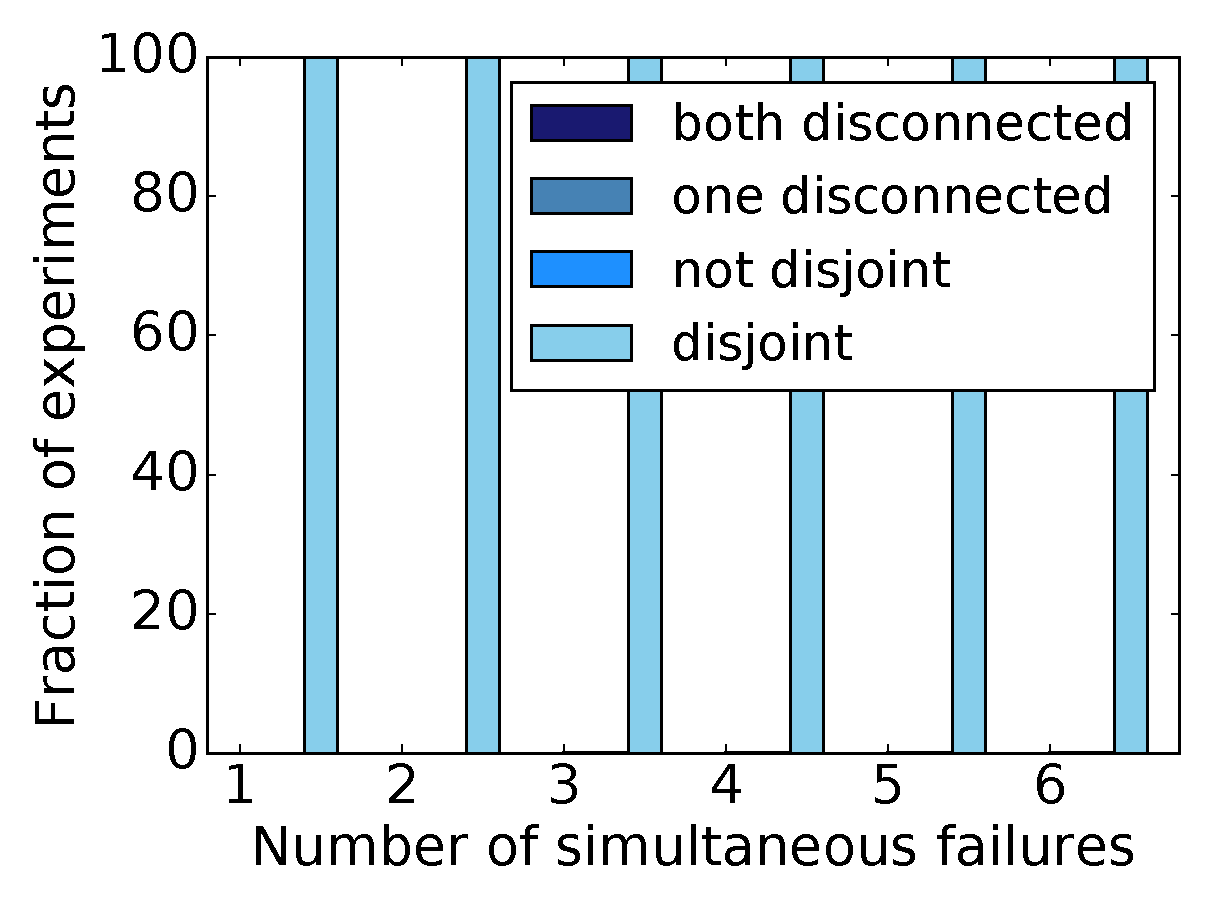
\includegraphics[width=0.45 \columnwidth]{figures/real1_random.eps}
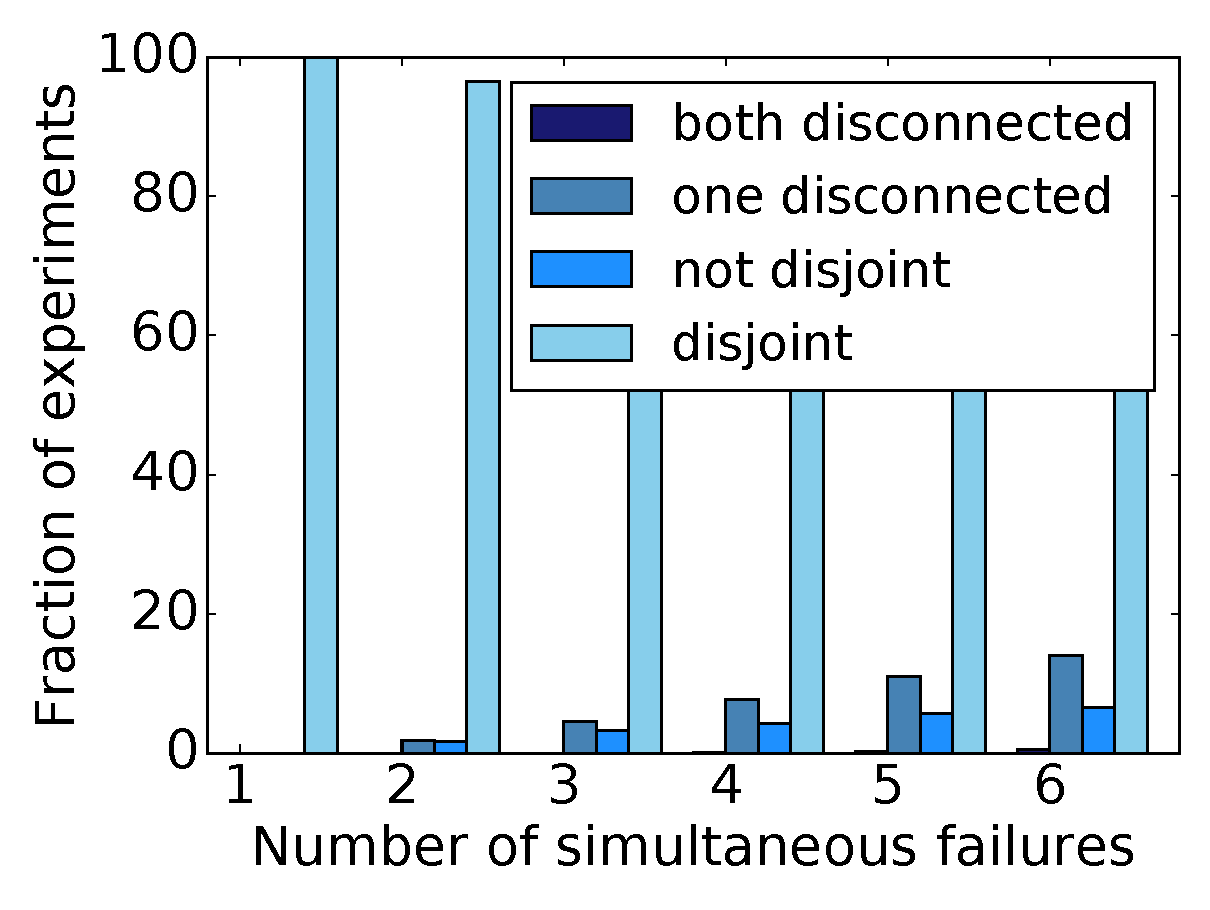
\includegraphics[width=0.45 \columnwidth]{figures/real1_worst.eps}
\end{center}
\caption{Random failures and path link failures over the worst case topoology.}
\label{fig:failure_sets_worst}
\end{figure}

\begin{figure}
\begin{center}
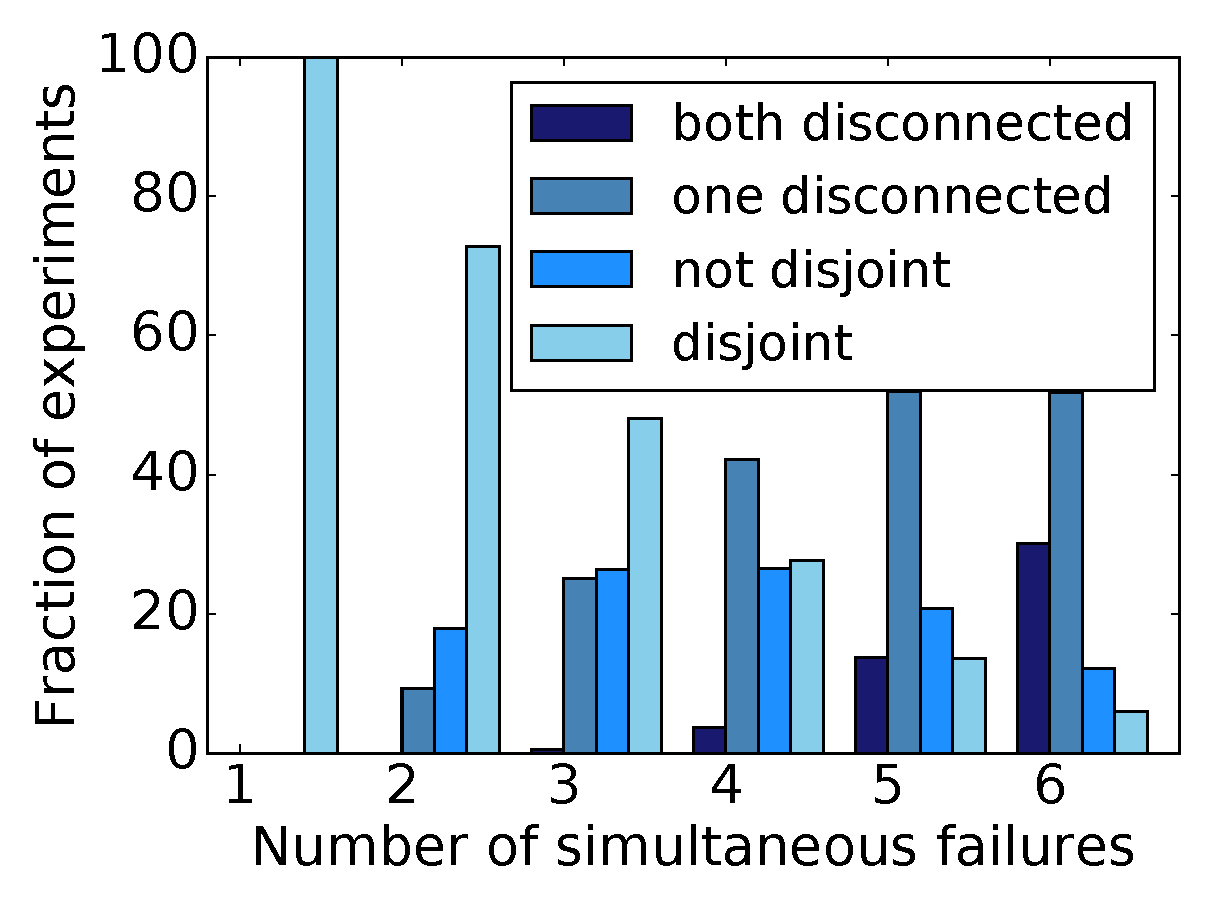
\includegraphics[width=0.45 \columnwidth]{figures/DialtelecomCz_worst.eps}
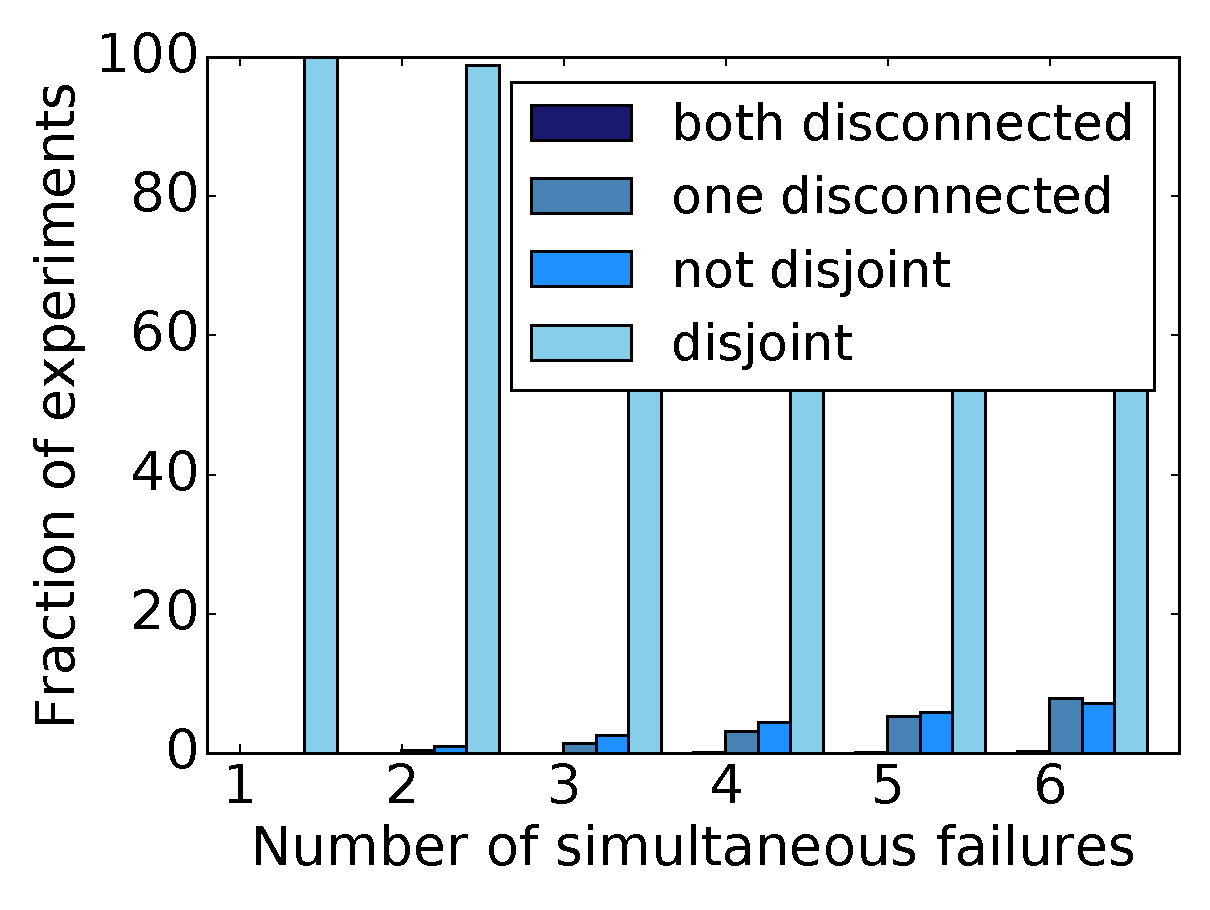
\includegraphics[width=0.45 \columnwidth]{figures/DialtelecomCz_random.eps}
\end{center}
\caption{Random failures and path link failures over the best case topology.}
\label{fig:failure_sets_best}
\end{figure}

We wondered whether we could evaluate the robustness of a pair of sr-paths algorithmically rather than 
having to perform such an experiment. The following theorem shows that it is $\NPhard$ to compute the minimum number of failures
that a pair of sr-paths can withstand until they cease to be disjoint.

\begin{problem}{Minimum cardinality failure}
\label{prob:eff-rob} 
\textbf{Input:} A network $G$ and two sr-paths $\sr{p}_1$ and $\sr{p}_2$.

\textbf{Output:} The cardinality of a minimal set of links $f \subseteq E(G)$ such that
$\sr{p}_1$ and $\sr{p}_2$ are not disjoint on $G \setminus f$.
\end{problem}

\begin{theorem}
Problem \ref{prob:eff-rob} is \NPhard. 
\end{theorem}

The following proof resulted from discussions with a student of mine, Simon Tihon, while I was coaching 
him for algorithmic programming contents.

\begin{proof}
To prove that this problem is $\NPhard$ it is enough to prove that the problem is $\NPhard$ for sr-paths of the form
$\sr{p}_1 = \langle s_1, t_1 \rangle$ and $\sr{p}_2 = \langle s_2, t_2 \rangle$. This amounts to,
given four nodes $s_1, s_2, t_1$ and $t_2$, find the minimum numbers of edges that we need to remove so that
the shortest paths from $s_1$ to $t_1$ intersect the shortest paths from $s_2$ to $t_2$.

It is known that the problem of finding the minimum number of edges that need to be removed so that the shortest path
between two given nodes becomes strictly larger than a given value $d$ is $\NPhard$ \cite{Golovach2011PathsOB}. Let $G, s, t, d$ be an instance
of this problem and assume that we can solve our problem
is polynomial time. We can assume that the shortest path between $s$ and $t$ has cost lower than or equal to $d$ or otherwise the problem is trivial.
e build an instance of Problem \ref{prob:eff-rob} by setting $s_2 = s, t_2 = t$ and adding two
nodes $s_1, t_1$. We connect $s_1$ to $s_2$ with an link of weight $d$ and $t_1$ to $t_2$ with a link of weight
$0$. Nodes $s_1$ and $t_1$ are connected with $K + 1$ parallel edges of weight $0$ where $K$ is the value of the
minimum cut between $s$ and $t$ on $G$. Figure \ref{fig:reduction} illustrates this construction.

\begin{figure}[H]
\begin{center}
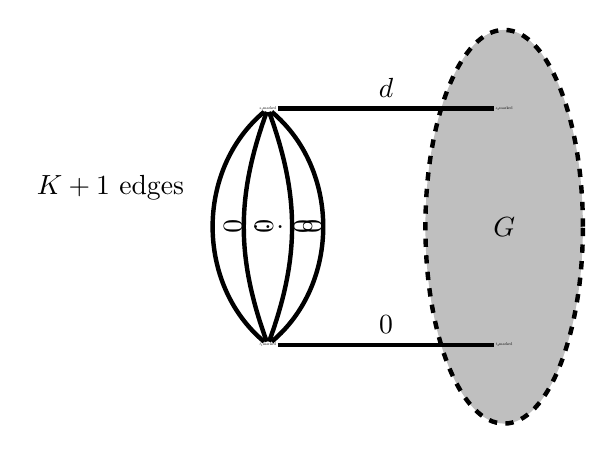
\begin{tikzpicture}
\draw[ultra thick, dashed, fill=gray!50!white] (3, -1.5) ellipse (1 and 2.5);

% \node[draw, circle, fill=lightgray] (s1) at (0, 0) {$s_1$};
% \node[draw, circle, fill=lightgray] (s2) at (3, 0) {$s_2$};
% \node[draw, circle, fill=lightgray] (t1) at (0, -3) {$t_1$};
% \node[draw, circle, fill=lightgray] (t2) at (3, -3) {$t_2$};

\node[scale=0.15] (s1) at (0,  0) {\router{$s_1$}{marked}};
\node[scale=0.15] (s2) at (3,  0) {\router{$s_2$}{marked}};
\node[scale=0.15] (t1) at (0,  -3) {\router{$t_1$}{marked}};
\node[scale=0.15] (t2) at (3,  -3) {\router{$t_2$}{marked}};


\draw (s1) edge[ultra thick, bend left = 50, sloped, above] node {$0$} (t1);
\draw (s1) edge[ultra thick, bend left = 20, sloped, above] node {$0$} (t1);
\draw (s1) edge[ultra thick, bend right = 50, sloped, above] node {$0$} (t1);
\draw (s1) edge[ultra thick, bend right = 20, sloped, above] node {$0$} (t1);

\node at (0, -1.5) {$\ldots$};

\node at (-2, -1) {$K + 1$ edges};


\draw (s1) edge[ultra thick, above] node {$d$} (s2);
\draw (t1) edge[ultra thick, above] node {$0$} (t2);


\node at (3, -1.5) {$G$};

\end{tikzpicture}
\end{center}
\caption{Construction used in the problem reduction.}
\label{fig:reduction}
\end{figure}

The shortest paths between $s_1$ and $t_1$ consists of the parallel links between them
whereas the shortest paths between $s_2 = s$ and $t_2 = t$ lie on $G$ since we assumed that the shortest
path from $s$ to $t$ has a cost lower than $d$. Note that the path visiting nodes $(s_2, s_1, t_1, t_2)$ has cost
$d$. Therefore, the shortest path from $s_2$ to $t_2$ will intersect the shortest paths from $s_1$ to $t_1$ if and only
if the shortest path from $s_1$ to $t_1$ on $G$ costs more than $d$.
Clearly, the minimum number of edges that we need to remove
so that the cost of the shortest path from $s$ to $t$ becomes at least $d$ is at most $K$ since $K$
is the value of a minimum cut (and thus a solution). Thus after removing this set the path are still well defined
since we have $K + 1$ parallel edges.
\end{proof}

\subsubsection{Evaluating existence and quality of RDPs}

In this section we will use the word detour to refer to an intermediate 
node that is in the segment stack. More concretely, for a sr-path of the form
$\langle x_1, x_2, \ldots, x_{n - 1}, x_n \rangle$, the detours are the nodes
$x_2, \ldots, x_{n - 1}$. Clearly a sr-path with $r$ detours has segment cost
$r + 2$.

We focus on reasonably well-connected \textit{source-destination
tuples}. For each topology, we randomly select 100 tuples $(s_1, s_2, t_1, t_2)$
of two sources $s_1,s_2$ and two destinations $t_1,t_2$, such that $s_1$ and
$s_2$ have a path to $t_1$ and $t_2$ even when any edge is removed. Since we try to
compute robustly disjoint paths from $s_1$ to $t_1$ and from $s_2$ to $t_2$,
it would indeed make little sense to consider source-destination pairs that are
disconnected by a single failure -- it is obvious that a service provider cannot offer
a robust connectivity service between routers that are poorly connected.
We repeat each experiment allowing between 1 and 3 detours ($k = 3, 4, 5$). We stop
at 3.

Table \ref{tab:rdp_existence} shows the percentage of these tuples for which robustly
disjoint paths exist. Sometimes, only selecting the right IGP paths is sufficient
for a given tuple. However, since IGP costs are shared across all
paths, they rarely can be used for more than one source-destination
tuple, preventing operators to configure robustly disjoint paths for
multiple customers or between different sites of the same customer.
Adding one detour by specifying an intermediate node with SR
allows paths for different tuples to be independent from each other,
solving the above issue. It also drastically increases the percentage
of tuples with at least one pair of robustly disjoint paths to 71%-100%
across all the topologies, and to 97% or more for all topologies but
two. Allowing more detours provides only slightly more flexibility
in our experiments.

\begin{figure}
\begin{center}
\begin{tabular}{ l | c c c c }
  \toprule
  & \multicolumn{3}{c}{Number of detours} \\
  Topology & 0 det & 1 det & 2 det & 3 det \\
  \midrule
  Real ISP 1 & 83\% & 100\% & 100\% & 100\% \\
  Real ISP 2 & 89\% & 100\% & 100\% & 100\% \\
  Real ISP 3 & 73\% & 100\% & 100\% & 100\% \\
  \midrule
  AS 1221 & 82\% & 98\% & 100\% & 100\% \\
  AS 1239 & 90\% & 100\% & 100\% & 100\% \\
  AS 1755 & 52\% & 98\% & 100\% & 100\% \\
  AS 3257 & 76\% & 100\% & 100\% & 100\% \\
  AS 3967 & 71\% & 99\% & 100\% & 100\% \\
  AS 6461 & 75\% & 100\% & 100\% & 100\% \\
  \midrule
  ITZ Cogentco & 78\% & 97\% & 100\% & 100\% \\ 
  ITZ Colt & 58\% & 71\% & 73\% & 73\% \\
  ITZ Deltacom & 74\% & 99\% & 99\% & 100\% \\
  ITZ Dia & 54\% & 77\% & 79\% & 79\% \\
  ITZ GtsCe & 78\% & 98\% & 100\% & 100\% \\
  ITZ Interoute & 81\% & 99\% & 100\% & 100\% \\
  ITZ Ion & 64\% & 100\% & 100\% & 100\% \\
  ITZ Tata & 86\% & 100\% & 100\% & 100\% \\
  ITZ UsCarrier & 72\% & 83\% & 85\% & 85\% \\
  \bottomrule
\end{tabular}
\end{center}
\caption{Percentage of tuples for which RDPs exist.}
\label{tab:rdp_existence}
\end{figure}

Our algorithms are designed to find sr-paths that are both
robustly disjoint and have minimal worst-path delay. As 
table \ref{tab:rdp_lat} shows, the robustly disjoint paths computed by our
algorithms have a worst-path delay which is always better than
the worst latency across the original IGP shortest paths. We are
up to 15\% more efficient, on average. Once again, more detours
enable to decrease the latency of the computed paths across all the
topologies, but just negligibly in most cases.

\begin{figure}
\begin{center}
\begin{tabular}{ l | c c c }
  \toprule
  & \multicolumn{3}{c}{Number of detours} \\
  Topology &  1 det & 2 det & 3 det \\
  \midrule
  Real ISP 1 & 0.97 & 0.97 & 0.97 \\
  Real ISP 2 & 0.98 & 0.98 & 0.98  \\
  Real ISP 3 & 0.97 & 0.96 & 0.96  \\
  \midrule
  AS 1221 & 0.99 & 0.99 & 0.99 \\
  AS 1239 & 0.97 & 0.97 & 0.97  \\
  AS 1755 & 0.90 & 0.89 & 0.88  \\
  AS 3257 & 0.91 & 0.89 & 0.88\\
  AS 3967 & 0.97 & 0.97 & 0.97  \\
  AS 6461 & 0.97 & 0.97 & 0.97  \\
  \midrule
  ITZ Cogentco & 0.85 & 0.84 & 0.84  \\ 
  ITZ Colt & 0.88 & 0.87 & 0.86  \\
  ITZ Deltacom & 0.91 & 0.90 & 0.90  \\
  ITZ Dia & 0.96 & 0.98 & 0.98  \\
  ITZ GtsCe & 0.78 & 0.77 & 0.75 \\
  ITZ Interoute & 0.93 & 0.91 & 0.90   \\
  ITZ Ion & 0.95 & 0.94 & 0.94  \\
  ITZ Tata & 0.90 & 0.89 & 0.89  \\
  ITZ UsCarrier & 0.92 & 0.92 & 0.92   \\
  \bottomrule
\end{tabular}
\end{center}
\caption{Average ratio between the RPD latency and the nominal latency.}
\label{tab:rdp_lat}
\end{figure}

To assess the benefits of robustly disjoint paths in a real-life scenario, 
we also analyse a 1-week trace of all the link-state IGP packets
exchanged by a router in Real ISP2. Based on this trace, we identified 
that a total of 5\% of the links failed during this period. Some
links experienced flapping, confirming observations of previous
studies [28, 45]. For example, one of the links failed more than 30
times during the analysed week. We select 100 source-destination
pairs in this network, and compute the corresponding robustly
disjoint paths for F = E (all single-link failures). We then replayed
all the failures that happened during the entire week. The 
source-destination pairs always have disjoint paths in our simulation, at
any moment during the week, even when multiple edges failed
simultaneously. This experiment provides a strong indication that
the paths computed by our algorithms are robust to real failures,
for a long time, in an operational network, without the need for
any configuration adjustment.
